% Options for packages loaded elsewhere
\PassOptionsToPackage{unicode}{hyperref}
\PassOptionsToPackage{hyphens}{url}
\documentclass[
]{article}
\usepackage{xcolor}
\usepackage[margin=1in]{geometry}
\usepackage{amsmath,amssymb}
\setcounter{secnumdepth}{-\maxdimen} % remove section numbering
\usepackage{iftex}
\ifPDFTeX
  \usepackage[T1]{fontenc}
  \usepackage[utf8]{inputenc}
  \usepackage{textcomp} % provide euro and other symbols
\else % if luatex or xetex
  \usepackage{unicode-math} % this also loads fontspec
  \defaultfontfeatures{Scale=MatchLowercase}
  \defaultfontfeatures[\rmfamily]{Ligatures=TeX,Scale=1}
\fi
\usepackage{lmodern}
\ifPDFTeX\else
  % xetex/luatex font selection
\fi
% Use upquote if available, for straight quotes in verbatim environments
\IfFileExists{upquote.sty}{\usepackage{upquote}}{}
\IfFileExists{microtype.sty}{% use microtype if available
  \usepackage[]{microtype}
  \UseMicrotypeSet[protrusion]{basicmath} % disable protrusion for tt fonts
}{}
\makeatletter
\@ifundefined{KOMAClassName}{% if non-KOMA class
  \IfFileExists{parskip.sty}{%
    \usepackage{parskip}
  }{% else
    \setlength{\parindent}{0pt}
    \setlength{\parskip}{6pt plus 2pt minus 1pt}}
}{% if KOMA class
  \KOMAoptions{parskip=half}}
\makeatother
\usepackage{color}
\usepackage{fancyvrb}
\newcommand{\VerbBar}{|}
\newcommand{\VERB}{\Verb[commandchars=\\\{\}]}
\DefineVerbatimEnvironment{Highlighting}{Verbatim}{commandchars=\\\{\}}
% Add ',fontsize=\small' for more characters per line
\usepackage{framed}
\definecolor{shadecolor}{RGB}{248,248,248}
\newenvironment{Shaded}{\begin{snugshade}}{\end{snugshade}}
\newcommand{\AlertTok}[1]{\textcolor[rgb]{0.94,0.16,0.16}{#1}}
\newcommand{\AnnotationTok}[1]{\textcolor[rgb]{0.56,0.35,0.01}{\textbf{\textit{#1}}}}
\newcommand{\AttributeTok}[1]{\textcolor[rgb]{0.13,0.29,0.53}{#1}}
\newcommand{\BaseNTok}[1]{\textcolor[rgb]{0.00,0.00,0.81}{#1}}
\newcommand{\BuiltInTok}[1]{#1}
\newcommand{\CharTok}[1]{\textcolor[rgb]{0.31,0.60,0.02}{#1}}
\newcommand{\CommentTok}[1]{\textcolor[rgb]{0.56,0.35,0.01}{\textit{#1}}}
\newcommand{\CommentVarTok}[1]{\textcolor[rgb]{0.56,0.35,0.01}{\textbf{\textit{#1}}}}
\newcommand{\ConstantTok}[1]{\textcolor[rgb]{0.56,0.35,0.01}{#1}}
\newcommand{\ControlFlowTok}[1]{\textcolor[rgb]{0.13,0.29,0.53}{\textbf{#1}}}
\newcommand{\DataTypeTok}[1]{\textcolor[rgb]{0.13,0.29,0.53}{#1}}
\newcommand{\DecValTok}[1]{\textcolor[rgb]{0.00,0.00,0.81}{#1}}
\newcommand{\DocumentationTok}[1]{\textcolor[rgb]{0.56,0.35,0.01}{\textbf{\textit{#1}}}}
\newcommand{\ErrorTok}[1]{\textcolor[rgb]{0.64,0.00,0.00}{\textbf{#1}}}
\newcommand{\ExtensionTok}[1]{#1}
\newcommand{\FloatTok}[1]{\textcolor[rgb]{0.00,0.00,0.81}{#1}}
\newcommand{\FunctionTok}[1]{\textcolor[rgb]{0.13,0.29,0.53}{\textbf{#1}}}
\newcommand{\ImportTok}[1]{#1}
\newcommand{\InformationTok}[1]{\textcolor[rgb]{0.56,0.35,0.01}{\textbf{\textit{#1}}}}
\newcommand{\KeywordTok}[1]{\textcolor[rgb]{0.13,0.29,0.53}{\textbf{#1}}}
\newcommand{\NormalTok}[1]{#1}
\newcommand{\OperatorTok}[1]{\textcolor[rgb]{0.81,0.36,0.00}{\textbf{#1}}}
\newcommand{\OtherTok}[1]{\textcolor[rgb]{0.56,0.35,0.01}{#1}}
\newcommand{\PreprocessorTok}[1]{\textcolor[rgb]{0.56,0.35,0.01}{\textit{#1}}}
\newcommand{\RegionMarkerTok}[1]{#1}
\newcommand{\SpecialCharTok}[1]{\textcolor[rgb]{0.81,0.36,0.00}{\textbf{#1}}}
\newcommand{\SpecialStringTok}[1]{\textcolor[rgb]{0.31,0.60,0.02}{#1}}
\newcommand{\StringTok}[1]{\textcolor[rgb]{0.31,0.60,0.02}{#1}}
\newcommand{\VariableTok}[1]{\textcolor[rgb]{0.00,0.00,0.00}{#1}}
\newcommand{\VerbatimStringTok}[1]{\textcolor[rgb]{0.31,0.60,0.02}{#1}}
\newcommand{\WarningTok}[1]{\textcolor[rgb]{0.56,0.35,0.01}{\textbf{\textit{#1}}}}
\usepackage{graphicx}
\makeatletter
\newsavebox\pandoc@box
\newcommand*\pandocbounded[1]{% scales image to fit in text height/width
  \sbox\pandoc@box{#1}%
  \Gscale@div\@tempa{\textheight}{\dimexpr\ht\pandoc@box+\dp\pandoc@box\relax}%
  \Gscale@div\@tempb{\linewidth}{\wd\pandoc@box}%
  \ifdim\@tempb\p@<\@tempa\p@\let\@tempa\@tempb\fi% select the smaller of both
  \ifdim\@tempa\p@<\p@\scalebox{\@tempa}{\usebox\pandoc@box}%
  \else\usebox{\pandoc@box}%
  \fi%
}
% Set default figure placement to htbp
\def\fps@figure{htbp}
\makeatother
\setlength{\emergencystretch}{3em} % prevent overfull lines
\providecommand{\tightlist}{%
  \setlength{\itemsep}{0pt}\setlength{\parskip}{0pt}}
\usepackage{bookmark}
\IfFileExists{xurl.sty}{\usepackage{xurl}}{} % add URL line breaks if available
\urlstyle{same}
% fallback for those not using the hyperref driver hyperxmp:
\makeatletter
\@ifundefined{xmpquote}{\newcommand{\xmpquote}[1]{#1}}{}
\makeatother
\hypersetup{
  pdftitle={Práctica 5. Datos Anómalos},
  hidelinks,
  pdfcreator={LaTeX via pandoc}}

\title{Práctica 5. Datos Anómalos}
\usepackage{etoolbox}
\makeatletter
\providecommand{\subtitle}[1]{% add subtitle to \maketitle
  \apptocmd{\@title}{\par {\large #1 \par}}{}{}
}
\makeatother
\subtitle{Análisis Exploratorio de Datos, Máster en Ciencia de Datos -
UV}
\author{}
\date{\vspace{-2.5em}}

\begin{document}
\maketitle

{
\setcounter{tocdepth}{3}
\tableofcontents
}
\begin{Shaded}
\begin{Highlighting}[]
\FunctionTok{library}\NormalTok{(pacman)}
\NormalTok{packages }\OtherTok{=} \FunctionTok{c}\NormalTok{(}\StringTok{"knitr"}\NormalTok{, }\StringTok{"ggplot2"}\NormalTok{,}\StringTok{"tidyr"}\NormalTok{,}\StringTok{"dplyr"}\NormalTok{,}\StringTok{"readr"}\NormalTok{)}
\NormalTok{pacman}\SpecialCharTok{::}\FunctionTok{p\_load}\NormalTok{(}\AttributeTok{char=}\NormalTok{packages)}
\end{Highlighting}
\end{Shaded}

\section{Introducción y objetivos}\label{introducciuxf3n-y-objetivos}

El objetivo de esta práctica es comprobar si los conjuntos de datos con
los que vamos a trabajar son consistentes y, por tanto, pueden ser
empleados para realizar un análisis sin errores. Las observaciones
contenidas en los datos pueden presentar diferentes tipos de
inconsistencias, como valores perdidos (missing values), valores
especiales y valores anómalos (outliers).

Para evitar estas inconsistencias, estos datos deberán ser eliminados,
corregidos o imputados. Siendo las etapas que pueden seguirse para
obtener datos consistentes:

\begin{enumerate}
\def\labelenumi{\arabic{enumi}.}
\tightlist
\item
  Detección de las inconsistencias.
\item
  Detectar el campo o campos que la generan y las dependencias entre
  ellos.
\item
  Corrección de errores.
\end{enumerate}

Vamos a trabajar con el conjunto de datos \emph{dirty\_iris}, que ya
conocemos, que contiene datos perdidos, valores especiales y anomalías
de carácter numérico respecto a la distribución de los datos
(\texttt{dirty\_iris.csv}).

\begin{Shaded}
\begin{Highlighting}[]
\FunctionTok{rm}\NormalTok{(}\AttributeTok{list=}\FunctionTok{ls}\NormalTok{())}
\NormalTok{dirty\_iris }\OtherTok{\textless{}{-}} \FunctionTok{read\_csv}\NormalTok{(}\StringTok{"data/dirty\_iris.csv"}\NormalTok{)}
\end{Highlighting}
\end{Shaded}

\section{Detección de inconsistencias en los
datos}\label{detecciuxf3n-de-inconsistencias-en-los-datos}

Por lo general, no hay un convenio o una representación común para
indicar un dato perdido o incluso determinados valores especiales. En
los siguientes ejercicios vamos a analizar cómo detectar inconsistencias
presentes en los datos.

\subsection{Ejercicio 1: Inspección
Visual}\label{ejercicio-1-inspecciuxf3n-visual}

Inspecciona visualmente los valores del conjunto de datos
(\texttt{View}) y ordena de mayor a menor y de menor a mayor cada
variable para descubrir las diferentes inconsistencias que presenta el
conjunto \texttt{dirty\_iris}. Comenta los valores que te llamen la
atención.

\begin{Shaded}
\begin{Highlighting}[]
\CommentTok{\# Medidas con valores faltantes, longitudes negativas y cero}
\CommentTok{\#View(dirty\_iris)}
\FunctionTok{summary}\NormalTok{(dirty\_iris)}
\end{Highlighting}
\end{Shaded}

\begin{verbatim}
  Sepal.Length     Sepal.Width      Petal.Length    Petal.Width    Species         
 Min.   : 0.000   Min.   :-3.000   Min.   : 0.00   Min.   :0.1   Length:150        
 1st Qu.: 5.100   1st Qu.: 2.800   1st Qu.: 1.60   1st Qu.:0.3   Class :character  
 Median : 5.750   Median : 3.000   Median : 4.50   Median :1.3   Mode  :character  
 Mean   : 6.559   Mean   : 3.391   Mean   : 4.45   Mean   :Inf                     
 3rd Qu.: 6.400   3rd Qu.: 3.300   3rd Qu.: 5.10   3rd Qu.:1.8                     
 Max.   :73.000   Max.   :30.000   Max.   :63.00   Max.   :Inf                     
 NA's   :10       NA's   :17       NA's   :19      NA's   :12                      
\end{verbatim}

\begin{Shaded}
\begin{Highlighting}[]
\ControlFlowTok{for}\NormalTok{ (v }\ControlFlowTok{in} \FunctionTok{names}\NormalTok{(dirty\_iris)[}\FunctionTok{sapply}\NormalTok{(dirty\_iris, is.numeric)]) \{}
  \FunctionTok{cat}\NormalTok{(}\StringTok{"}\SpecialCharTok{\textbackslash{}n}\StringTok{=========="}\NormalTok{, v, }\StringTok{"==========}\SpecialCharTok{\textbackslash{}n}\StringTok{"}\NormalTok{)}
  \FunctionTok{cat}\NormalTok{(}\StringTok{"Valores más pequeños:}\SpecialCharTok{\textbackslash{}n}\StringTok{"}\NormalTok{)}
  \FunctionTok{print}\NormalTok{(dirty\_iris }\SpecialCharTok{\%\textgreater{}\%} \FunctionTok{arrange}\NormalTok{(.data[[v]]) }\SpecialCharTok{\%\textgreater{}\%} \FunctionTok{select}\NormalTok{(}\FunctionTok{all\_of}\NormalTok{(v), Species) }\SpecialCharTok{\%\textgreater{}\%} \FunctionTok{head}\NormalTok{(}\DecValTok{5}\NormalTok{))}
  \FunctionTok{cat}\NormalTok{(}\StringTok{"Valores más grandes:}\SpecialCharTok{\textbackslash{}n}\StringTok{"}\NormalTok{)}
  \FunctionTok{print}\NormalTok{(dirty\_iris }\SpecialCharTok{\%\textgreater{}\%} \FunctionTok{arrange}\NormalTok{(}\FunctionTok{desc}\NormalTok{(.data[[v]])) }\SpecialCharTok{\%\textgreater{}\%} \FunctionTok{select}\NormalTok{(}\FunctionTok{all\_of}\NormalTok{(v), Species) }\SpecialCharTok{\%\textgreater{}\%} \FunctionTok{head}\NormalTok{(}\DecValTok{5}\NormalTok{))}
\NormalTok{\}}
\end{Highlighting}
\end{Shaded}

\begin{verbatim}

========== Sepal.Length ==========
Valores más pequeños:
# A tibble: 5 x 2
  Sepal.Length Species
         <dbl> <chr>  
1          0   setosa 
2          4.3 setosa 
3          4.4 setosa 
4          4.4 setosa 
5          4.4 setosa 
Valores más grandes:
# A tibble: 5 x 2
  Sepal.Length Species  
         <dbl> <chr>    
1         73   virginica
2         49   setosa   
3          7.9 virginica
4          7.7 virginica
5          7.7 virginica

========== Sepal.Width ==========
Valores más pequeños:
# A tibble: 5 x 2
  Sepal.Width Species   
        <dbl> <chr>     
1        -3   versicolor
2         0   setosa    
3         2.2 versicolor
4         2.2 virginica 
5         2.2 versicolor
Valores más grandes:
# A tibble: 5 x 2
  Sepal.Width Species  
        <dbl> <chr>    
1        30   setosa   
2        29   virginica
3         4.2 setosa   
4         4.1 setosa   
5         4   setosa   

========== Petal.Length ==========
Valores más pequeños:
# A tibble: 5 x 2
  Petal.Length Species   
         <dbl> <chr>     
1        0     setosa    
2        0.82  versicolor
3        0.925 versicolor
4        1.1   setosa    
5        1.2   setosa    
Valores más grandes:
# A tibble: 5 x 2
  Petal.Length Species   
         <dbl> <chr>     
1         63   virginica 
2         23   versicolor
3         14   setosa    
4          6.9 virginica 
5          6.7 virginica 

========== Petal.Width ==========
Valores más pequeños:
# A tibble: 5 x 2
  Petal.Width Species
        <dbl> <chr>  
1         0.1 setosa 
2         0.1 setosa 
3         0.1 setosa 
4         0.1 setosa 
5         0.1 setosa 
Valores más grandes:
# A tibble: 5 x 2
  Petal.Width Species  
        <dbl> <chr>    
1       Inf   setosa   
2         2.5 virginica
3         2.5 virginica
4         2.5 virginica
5         2.4 virginica
\end{verbatim}

\begin{Shaded}
\begin{Highlighting}[]
\CommentTok{\# Registros con valores de otra escala (filas completas muy por encima del resto)}
\NormalTok{dirty\_iris }\SpecialCharTok{\%\textgreater{}\%} \FunctionTok{filter}\NormalTok{(Sepal.Length }\SpecialCharTok{\textgreater{}} \DecValTok{10} \SpecialCharTok{|}\NormalTok{ Sepal.Width }\SpecialCharTok{\textgreater{}} \DecValTok{10} \SpecialCharTok{|}\NormalTok{ Petal.Length }\SpecialCharTok{\textgreater{}} \DecValTok{10}\NormalTok{)}
\end{Highlighting}
\end{Shaded}

\begin{verbatim}
# A tibble: 3 x 5
  Sepal.Length Sepal.Width Petal.Length Petal.Width Species   
         <dbl>       <dbl>        <dbl>       <dbl> <chr>     
1         73          29             63        NA   virginica 
2          6.6         2.9           23         1.3 versicolor
3         49          30             14         2   setosa    
\end{verbatim}

Hay bastantes valores perdidos (\texttt{NA}) en las cuatro variables
numéricas. \texttt{Sepal.Width} tiene un valor \textbf{negativo} (-3),
imposible para una longitud.

Hay valores \textbf{iguales a cero} en \texttt{Sepal.Length},
\texttt{Sepal.Width} y \texttt{Petal.Length}, también imposibles para
medidas de una flor.

\texttt{Petal.Width} contiene un valor \textbf{infinito} (\texttt{Inf}).

Hay filas con valores de otra escala (73, 29, 63 en una virginica y 49,
30, 14 en una setosa), que parecen errores de unidades (valores
multiplicados por 10).

\texttt{Petal.Length} también tiene un 23 en una versicolor, muy alejado
del resto, y valores muy pequeños e implausibles para una versicolor
(0.82 y 0.925).

\subsection{Ejercicio 2: Valores
especiales}\label{ejercicio-2-valores-especiales}

Visualizar los datos puede ser muy revelador, pero en general,
especialmente para conjuntos de datos grandes, realizaremos este
análisis de forma automática.

Los valores especiales más comunes en R son:

\begin{itemize}
\tightlist
\item
  NA (\emph{not available}): missing value o dato perdido
  (\texttt{is.na})
\item
  NULL (\emph{empty set}): elemento nulo de longitud 0
  (\texttt{is.null})
\item
  NaN (\emph{not a number}): indeterminación con resultado desconocido
  (\texttt{is.nan})
\item
  Inf (\emph{infinite}): valor numérico de valor infinito
  (\texttt{is.infinite})
\end{itemize}

Nota: A parte de estas funciones, \texttt{is.numeric} comprueba si la
variable es numérica; \texttt{is.finite} comprueba la existencia de
cualquier valor especial en un vector numérico pero devuelve
\texttt{FALSE} para variables de texto.

Reemplaza, en todas las columnas numéricas del data frame
\texttt{dirty\_iris}, los valores que sean especiales (usando
\texttt{is.finite}), negativos, o iguales a cero, por \texttt{NA}. Nota:
Puedes reemplazar los valores para cada variable del dataframe usando
\texttt{mutate} con la función \texttt{ifelse}.

\begin{Shaded}
\begin{Highlighting}[]
\NormalTok{dirty\_iris }\OtherTok{\textless{}{-}}\NormalTok{ dirty\_iris }\SpecialCharTok{\%\textgreater{}\%}
  \FunctionTok{mutate}\NormalTok{(}\FunctionTok{across}\NormalTok{(}\FunctionTok{where}\NormalTok{(is.numeric),}
                \SpecialCharTok{\textasciitilde{}} \FunctionTok{ifelse}\NormalTok{(}\FunctionTok{is.finite}\NormalTok{(.x) }\SpecialCharTok{\&}\NormalTok{ .x }\SpecialCharTok{\textgreater{}} \DecValTok{0}\NormalTok{, .x, }\ConstantTok{NA}\NormalTok{)))}

\FunctionTok{colSums}\NormalTok{(}\FunctionTok{is.na}\NormalTok{(dirty\_iris))}
\end{Highlighting}
\end{Shaded}

\begin{verbatim}
Sepal.Length  Sepal.Width Petal.Length  Petal.Width      Species 
          11           19           20           13            0 
\end{verbatim}

\subsection{Ejercicio 3: Valores perdidos y observaciones
completas}\label{ejercicio-3-valores-perdidos-y-observaciones-completas}

\begin{itemize}
\tightlist
\item
  Calcula el número y porcentaje de observaciones completas (muestras
  sin ningún dato perdido) empleando \texttt{complete.cases} (detecta
  todos los registros sin datos faltantes).
\item
  Emplea después la función \texttt{na.omit} para quedarnos solo con las
  filas con datos completos en un nuevo data frame \texttt{clean\_iris}.
\end{itemize}

\begin{Shaded}
\begin{Highlighting}[]
\NormalTok{n\_completas }\OtherTok{\textless{}{-}} \FunctionTok{sum}\NormalTok{(}\FunctionTok{complete.cases}\NormalTok{(dirty\_iris))}
\NormalTok{pct\_completas }\OtherTok{\textless{}{-}} \DecValTok{100} \SpecialCharTok{*}\NormalTok{ n\_completas }\SpecialCharTok{/} \FunctionTok{nrow}\NormalTok{(dirty\_iris)}
\FunctionTok{cat}\NormalTok{(}\StringTok{"Observaciones completas:"}\NormalTok{, n\_completas, }\StringTok{"de"}\NormalTok{, }\FunctionTok{nrow}\NormalTok{(dirty\_iris),}
    \StringTok{"("}\NormalTok{, }\FunctionTok{round}\NormalTok{(pct\_completas, }\DecValTok{2}\NormalTok{), }\StringTok{"\% )}\SpecialCharTok{\textbackslash{}n}\StringTok{"}\NormalTok{)}
\end{Highlighting}
\end{Shaded}

\begin{verbatim}
Observaciones completas: 92 de 150 ( 61.33 % )
\end{verbatim}

\begin{Shaded}
\begin{Highlighting}[]
\NormalTok{clean\_iris }\OtherTok{\textless{}{-}} \FunctionTok{na.omit}\NormalTok{(dirty\_iris)}
\FunctionTok{dim}\NormalTok{(clean\_iris)}
\end{Highlighting}
\end{Shaded}

\begin{verbatim}
[1] 92  5
\end{verbatim}

\section{Detección de outliers
univariante}\label{detecciuxf3n-de-outliers-univariante}

Un outlier es una observación (o conjunto de observaciones) que no
parecen consistentes con el resto de valores de esa variable. Por lo
general, esas observaciones divergirán del patrón de comportamiento del
resto de datos, es decir, presentarán una desviación respecto de la
distribución de los datos.

En esta sección, vamos a centrarnos en métodos de detección
univariantes, así que, en los ejercicios, a modo de ejemplo,
analizaremos solo la variable \texttt{Petal.Length}.

\subsection{Ejercicio 4: Estadísticos
básicos}\label{ejercicio-4-estaduxedsticos-buxe1sicos}

La presencia de outliers puede producir una gran influencia en
caracterizaciones sencillas de los datos, como la media y la desviación
típica.

Empleado la función \texttt{summarise\ y\ across}, calcula la media, la
desviación típica, mediana, la \emph{median absolute deviation from the
median} (MADM) y el \emph{interquartile range} (IQR) de las variables
numéricas. Hazlo para el data frame con observaciones completas
\texttt{clean\_iris} (que no tiene NA pero tiene menos observaciones) y
para el data frame con datos faltantes \texttt{dirty\_iris} (que
presenta muchos NA pero tiene todas las observaciones).

\begin{itemize}
\tightlist
\item
  Ten en cuenta que no se puede realizar un análisis estadístico con
  datos faltantes, pero en la mayoría de los casos se puede optar por no
  considerar dichos valores al realizar los cálculos (parámetro
  \texttt{na.rm=TRUE}).
\item
  Para obtener el valor MADM, escribe una función \texttt{madm(x)} que
  sea robusta a la presencia de valores NA. Recuerda que el MADM se
  calcula como \(1.4826\cdot\textrm{median}(|x - \textrm{median(x)}|)\).
\item
  Compara los resultados para los dos conjuntos en la variable
  \texttt{Petal.Length}.
\end{itemize}

\begin{Shaded}
\begin{Highlighting}[]
\CommentTok{\#MADM=1.4826*median(∣x\_i −median(x)∣)}
\NormalTok{madm }\OtherTok{\textless{}{-}} \ControlFlowTok{function}\NormalTok{(x) \{}
  \FloatTok{1.4826} \SpecialCharTok{*} \FunctionTok{median}\NormalTok{(}\FunctionTok{abs}\NormalTok{(x }\SpecialCharTok{{-}} \FunctionTok{median}\NormalTok{(x, }\AttributeTok{na.rm =} \ConstantTok{TRUE}\NormalTok{)), }\AttributeTok{na.rm =} \ConstantTok{TRUE}\NormalTok{)}
\NormalTok{\}}

\CommentTok{\# Estadísticos básicos de todas las variables numéricas}
\NormalTok{estadisticos }\OtherTok{\textless{}{-}} \ControlFlowTok{function}\NormalTok{(df) \{}
\NormalTok{  df }\SpecialCharTok{\%\textgreater{}\%}
    \FunctionTok{summarise}\NormalTok{(}\FunctionTok{across}\NormalTok{(}\FunctionTok{where}\NormalTok{(is.numeric),}
                     \FunctionTok{list}\NormalTok{(}\AttributeTok{media   =} \SpecialCharTok{\textasciitilde{}} \FunctionTok{mean}\NormalTok{(.x, }\AttributeTok{na.rm =} \ConstantTok{TRUE}\NormalTok{),}
                          \AttributeTok{sd      =} \SpecialCharTok{\textasciitilde{}} \FunctionTok{sd}\NormalTok{(.x, }\AttributeTok{na.rm =} \ConstantTok{TRUE}\NormalTok{),}
                          \AttributeTok{mediana =} \SpecialCharTok{\textasciitilde{}} \FunctionTok{median}\NormalTok{(.x, }\AttributeTok{na.rm =} \ConstantTok{TRUE}\NormalTok{),}
                          \AttributeTok{madm    =} \SpecialCharTok{\textasciitilde{}} \FunctionTok{madm}\NormalTok{(.x),}
                          \AttributeTok{iqr     =} \SpecialCharTok{\textasciitilde{}} \FunctionTok{IQR}\NormalTok{(.x, }\AttributeTok{na.rm =} \ConstantTok{TRUE}\NormalTok{)),}
                     \AttributeTok{.names =} \StringTok{"\{.col\}\_\_\{.fn\}"}\NormalTok{)) }\SpecialCharTok{\%\textgreater{}\%}
    \FunctionTok{pivot\_longer}\NormalTok{(}\FunctionTok{everything}\NormalTok{(), }\AttributeTok{names\_to =} \FunctionTok{c}\NormalTok{(}\StringTok{"variable"}\NormalTok{, }\StringTok{"estadistico"}\NormalTok{),}
                 \AttributeTok{names\_sep =} \StringTok{"\_\_"}\NormalTok{) }\SpecialCharTok{\%\textgreater{}\%}
    \FunctionTok{pivot\_wider}\NormalTok{(}\AttributeTok{names\_from =}\NormalTok{ estadistico, }\AttributeTok{values\_from =}\NormalTok{ value)}
\NormalTok{\}}

\FunctionTok{cat}\NormalTok{(}\StringTok{"Observaciones completas (clean\_iris):}\SpecialCharTok{\textbackslash{}n}\StringTok{"}\NormalTok{)}
\end{Highlighting}
\end{Shaded}

\begin{verbatim}
Observaciones completas (clean_iris):
\end{verbatim}

\begin{Shaded}
\begin{Highlighting}[]
\NormalTok{est\_clean }\OtherTok{\textless{}{-}} \FunctionTok{estadisticos}\NormalTok{(clean\_iris)}
\NormalTok{est\_clean}
\end{Highlighting}
\end{Shaded}

\begin{verbatim}
# A tibble: 4 x 6
  variable     media    sd mediana  madm   iqr
  <chr>        <dbl> <dbl>   <dbl> <dbl> <dbl>
1 Sepal.Length  6.37 4.57      5.8 1.04    1.3
2 Sepal.Width   3.33 2.84      3   0.371   0.5
3 Petal.Length  4.16 2.88      4.5 1.63    3.6
4 Petal.Width   1.22 0.765     1.4 0.890   1.6
\end{verbatim}

\begin{Shaded}
\begin{Highlighting}[]
\FunctionTok{cat}\NormalTok{(}\StringTok{"}\SpecialCharTok{\textbackslash{}n}\StringTok{Datos con NA, todas las observaciones (dirty\_iris):}\SpecialCharTok{\textbackslash{}n}\StringTok{"}\NormalTok{)}
\end{Highlighting}
\end{Shaded}

\begin{verbatim}

Datos con NA, todas las observaciones (dirty_iris):
\end{verbatim}

\begin{Shaded}
\begin{Highlighting}[]
\NormalTok{est\_dirty }\OtherTok{\textless{}{-}} \FunctionTok{estadisticos}\NormalTok{(dirty\_iris)}
\NormalTok{est\_dirty}
\end{Highlighting}
\end{Shaded}

\begin{verbatim}
# A tibble: 4 x 6
  variable     media    sd mediana  madm   iqr
  <chr>        <dbl> <dbl>   <dbl> <dbl> <dbl>
1 Sepal.Length  6.61 6.80      5.8 1.04    1.3
2 Sepal.Width   3.47 3.28      3   0.297   0.5
3 Petal.Length  4.48 5.78      4.5 1.63    3.5
4 Petal.Width   1.21 0.765     1.3 1.04    1.5
\end{verbatim}

\begin{Shaded}
\begin{Highlighting}[]
\CommentTok{\# Comparación para Petal.Length}
\FunctionTok{bind\_rows}\NormalTok{(}\AttributeTok{clean\_iris =}\NormalTok{ est\_clean, }\AttributeTok{dirty\_iris =}\NormalTok{ est\_dirty, }\AttributeTok{.id =} \StringTok{"conjunto"}\NormalTok{) }\SpecialCharTok{\%\textgreater{}\%}
  \FunctionTok{filter}\NormalTok{(variable }\SpecialCharTok{==} \StringTok{"Petal.Length"}\NormalTok{)}
\end{Highlighting}
\end{Shaded}

\begin{verbatim}
# A tibble: 2 x 7
  conjunto   variable     media    sd mediana  madm   iqr
  <chr>      <chr>        <dbl> <dbl>   <dbl> <dbl> <dbl>
1 clean_iris Petal.Length  4.16  2.88     4.5  1.63   3.6
2 dirty_iris Petal.Length  4.48  5.78     4.5  1.63   3.5
\end{verbatim}

La media y la desviación típica de \texttt{Petal.Length} cambian
bastante entre los dos conjuntos (la media pasa de 4.16 a 4.48 y la
desviación típica de 2.88 a 5.78), porque los outliers (63, 23 y 14)
están en \texttt{dirty\_iris} y distorsionan esos estadísticos; en
\texttt{clean\_iris} se han descartado algunos de ellos al eliminar
filas con otros \texttt{NA}. En cambio la mediana (4.5), el MADM y el
IQR apenas varían, ya que son estadísticos robustos frente a outliers.

\subsection{Ejercicio 5: Métodos de detección de
outliers}\label{ejercicio-5-muxe9todos-de-detecciuxf3n-de-outliers}

Escribe una función que detecte los outliers de un vector \(x\) para
cada uno de los siguientes métodos de detección de outliers univariantes
(todas las funciones tienen que ser robustas a la presencia de valores
NA).

\begin{itemize}
\item
  \textbf{Regla 3 sigma} \texttt{reglasigma(x)}: Considera que los datos
  siguen una distribución gaussiana. Datos típicos caracterizados por la
  media y la dispersión por la varianza. Valores por encima de 3
  desviaciones típicas se consideran outliers.
\item
  \textbf{Identificador Hampel} \texttt{reglahampel(x)}: Utiliza
  estimadores robustos y no presupone que los datos siguen una
  distribución gaussiana. Datos típicos caracterizados por la mediana y
  la dispersión por la \emph{median absolute deviation from the median}
  (MADM). Valores por encima de 3 MADM se consideran outliers.
\item
  \textbf{Regla boxplot} \texttt{reglaboxplot(x)}: A partir de los datos
  se calcula su diagrama de caja (boxplot) y se definen como datos
  típicos superiores hasta el cuartil 75\%, \(x_s\); datos típicos
  inferiores hasta el cuartil 25\%, \(x_i\); y la dispersión se define
  como el rango intercuartílico (\(IQR= x_s-x_i\)). Valores por encima
  de \(x_s+1.5\cdot IQR\) o por debajo de \(x_i-1.5\cdot IQR\) se
  consideran outliers. Usa la función \texttt{quantile} para calcular
  los cuartiles.
\item
  \textbf{Percentiles} \texttt{reglapercentil(x)}: Cualquier valor que
  esté fuera del rango del percentil 5\% y 95\% se puede considerar como
  atípico. Usa la función \texttt{quantile} para calcular los
  percentiles.
\end{itemize}

\begin{Shaded}
\begin{Highlighting}[]
\CommentTok{\# Todas las funciones devuelven un vector lógico (TRUE = outlier);}
\CommentTok{\# si x es NA el resultado es NA.}

\CommentTok{\# Regla 3 sigma}
\NormalTok{reglasigma }\OtherTok{\textless{}{-}} \ControlFlowTok{function}\NormalTok{(x) \{}
  \FunctionTok{abs}\NormalTok{(x }\SpecialCharTok{{-}} \FunctionTok{mean}\NormalTok{(x, }\AttributeTok{na.rm =} \ConstantTok{TRUE}\NormalTok{)) }\SpecialCharTok{\textgreater{}} \DecValTok{3} \SpecialCharTok{*} \FunctionTok{sd}\NormalTok{(x, }\AttributeTok{na.rm =} \ConstantTok{TRUE}\NormalTok{)}
\NormalTok{\}}

\CommentTok{\# Identificador Hampel}
\NormalTok{reglahampel }\OtherTok{\textless{}{-}} \ControlFlowTok{function}\NormalTok{(x) \{}
  \FunctionTok{abs}\NormalTok{(x }\SpecialCharTok{{-}} \FunctionTok{median}\NormalTok{(x, }\AttributeTok{na.rm =} \ConstantTok{TRUE}\NormalTok{)) }\SpecialCharTok{\textgreater{}} \DecValTok{3} \SpecialCharTok{*} \FunctionTok{madm}\NormalTok{(x)}
\NormalTok{\}}

\CommentTok{\# Regla boxplot}
\NormalTok{reglaboxplot }\OtherTok{\textless{}{-}} \ControlFlowTok{function}\NormalTok{(x) \{}
\NormalTok{  q }\OtherTok{\textless{}{-}} \FunctionTok{quantile}\NormalTok{(x, }\AttributeTok{probs =} \FunctionTok{c}\NormalTok{(}\FloatTok{0.25}\NormalTok{, }\FloatTok{0.75}\NormalTok{), }\AttributeTok{na.rm =} \ConstantTok{TRUE}\NormalTok{, }\AttributeTok{names =} \ConstantTok{FALSE}\NormalTok{)}
\NormalTok{  iqr }\OtherTok{\textless{}{-}}\NormalTok{ q[}\DecValTok{2}\NormalTok{] }\SpecialCharTok{{-}}\NormalTok{ q[}\DecValTok{1}\NormalTok{]}
\NormalTok{  x }\SpecialCharTok{\textless{}}\NormalTok{ q[}\DecValTok{1}\NormalTok{] }\SpecialCharTok{{-}} \FloatTok{1.5} \SpecialCharTok{*}\NormalTok{ iqr }\SpecialCharTok{|}\NormalTok{ x }\SpecialCharTok{\textgreater{}}\NormalTok{ q[}\DecValTok{2}\NormalTok{] }\SpecialCharTok{+} \FloatTok{1.5} \SpecialCharTok{*}\NormalTok{ iqr}
\NormalTok{\}}

\CommentTok{\# Percentiles}
\NormalTok{reglapercentil }\OtherTok{\textless{}{-}} \ControlFlowTok{function}\NormalTok{(x) \{}
\NormalTok{  q }\OtherTok{\textless{}{-}} \FunctionTok{quantile}\NormalTok{(x, }\AttributeTok{probs =} \FunctionTok{c}\NormalTok{(}\FloatTok{0.05}\NormalTok{, }\FloatTok{0.95}\NormalTok{), }\AttributeTok{na.rm =} \ConstantTok{TRUE}\NormalTok{, }\AttributeTok{names =} \ConstantTok{FALSE}\NormalTok{)}
\NormalTok{  x }\SpecialCharTok{\textless{}}\NormalTok{ q[}\DecValTok{1}\NormalTok{] }\SpecialCharTok{|}\NormalTok{ x }\SpecialCharTok{\textgreater{}}\NormalTok{ q[}\DecValTok{2}\NormalTok{]}
\NormalTok{\}}
\end{Highlighting}
\end{Shaded}

\subsection{Ejercicio 6: Detección de
outliers}\label{ejercicio-6-detecciuxf3n-de-outliers}

Utiliza la función \texttt{mutate} y \texttt{across} para identificar
los outliers en la variable \texttt{Petal.Length} con todos los métodos
de detección de outliers implementados. Genera una columna nueva para
cada método. Nota: podría extenderse la aplicación a todas las variables
numéricas usando también \texttt{mutate}, \texttt{across} y
\texttt{where}.

\begin{Shaded}
\begin{Highlighting}[]
\NormalTok{iris\_out }\OtherTok{\textless{}{-}}\NormalTok{ dirty\_iris }\SpecialCharTok{\%\textgreater{}\%}
  \FunctionTok{mutate}\NormalTok{(}\FunctionTok{across}\NormalTok{(Petal.Length,}
                \FunctionTok{list}\NormalTok{(}\AttributeTok{sigma     =}\NormalTok{ reglasigma,}
                     \AttributeTok{hampel    =}\NormalTok{ reglahampel,}
                     \AttributeTok{boxplot   =}\NormalTok{ reglaboxplot,}
                     \AttributeTok{percentil =}\NormalTok{ reglapercentil),}
                \AttributeTok{.names =} \StringTok{"out\_\{.fn\}"}\NormalTok{))}

\NormalTok{iris\_out }\SpecialCharTok{\%\textgreater{}\%} \FunctionTok{select}\NormalTok{(Petal.Length, }\FunctionTok{starts\_with}\NormalTok{(}\StringTok{"out\_"}\NormalTok{)) }\SpecialCharTok{\%\textgreater{}\%} \FunctionTok{head}\NormalTok{(}\DecValTok{10}\NormalTok{)}
\end{Highlighting}
\end{Shaded}

\begin{verbatim}
# A tibble: 10 x 5
   Petal.Length out_sigma out_hampel out_boxplot out_percentil
          <dbl> <lgl>     <lgl>      <lgl>       <lgl>        
 1          4.5 FALSE     FALSE      FALSE       FALSE        
 2          6   FALSE     FALSE      FALSE       FALSE        
 3          5.4 FALSE     FALSE      FALSE       FALSE        
 4          1.6 FALSE     FALSE      FALSE       FALSE        
 5          3.5 FALSE     FALSE      FALSE       FALSE        
 6         NA   NA        NA         NA          NA           
 7          5.3 FALSE     FALSE      FALSE       FALSE        
 8          5.1 FALSE     FALSE      FALSE       FALSE        
 9          4.1 FALSE     FALSE      FALSE       FALSE        
10          1.6 FALSE     FALSE      FALSE       FALSE        
\end{verbatim}

\subsection{Ejercicio 7: Comparativa de los métodos de detección de
outliers}\label{ejercicio-7-comparativa-de-los-muxe9todos-de-detecciuxf3n-de-outliers}

En los métodos de detección de outliers analizados, examina los
resultados comparando:

\begin{itemize}
\tightlist
\item
  Número de outliers detectados por método.
\item
  Los valores etiquetados como outliers (ordenados de menor a mayor).
\end{itemize}

\begin{Shaded}
\begin{Highlighting}[]
\CommentTok{\# Número de outliers por método}
\NormalTok{iris\_out }\SpecialCharTok{\%\textgreater{}\%}
  \FunctionTok{summarise}\NormalTok{(}\FunctionTok{across}\NormalTok{(}\FunctionTok{starts\_with}\NormalTok{(}\StringTok{"out\_"}\NormalTok{), }\SpecialCharTok{\textasciitilde{}} \FunctionTok{sum}\NormalTok{(.x, }\AttributeTok{na.rm =} \ConstantTok{TRUE}\NormalTok{)))}
\end{Highlighting}
\end{Shaded}

\begin{verbatim}
# A tibble: 1 x 4
  out_sigma out_hampel out_boxplot out_percentil
      <int>      <int>       <int>         <int>
1         2          3           3            11
\end{verbatim}

\begin{Shaded}
\begin{Highlighting}[]
\CommentTok{\# Valores etiquetados como outliers por cada método (de menor a mayor)}
\NormalTok{reglas }\OtherTok{\textless{}{-}} \FunctionTok{grep}\NormalTok{(}\StringTok{"\^{}out\_"}\NormalTok{, }\FunctionTok{names}\NormalTok{(iris\_out), }\AttributeTok{value =} \ConstantTok{TRUE}\NormalTok{)}
\NormalTok{valores\_outliers }\OtherTok{\textless{}{-}} \FunctionTok{lapply}\NormalTok{(reglas, }\ControlFlowTok{function}\NormalTok{(r) \{}
  \FunctionTok{sort}\NormalTok{(iris\_out}\SpecialCharTok{$}\NormalTok{Petal.Length[iris\_out[[r]] }\SpecialCharTok{\%in\%} \ConstantTok{TRUE}\NormalTok{])}
\NormalTok{\})}
\CommentTok{\#iris\_out[[r]] \%in\% TRUE = que elementos de esa columna son true}
\CommentTok{\#iris\_out$Petal.Length[iris\_out[[r]] \%in\% TRUE] = devuelve los valores de Petal.Length que tienen true, es decir, son outliers}
\FunctionTok{names}\NormalTok{(valores\_outliers) }\OtherTok{\textless{}{-}} \FunctionTok{sub}\NormalTok{(}\StringTok{"\^{}out\_"}\NormalTok{, }\StringTok{""}\NormalTok{, reglas)}
\NormalTok{valores\_outliers}
\end{Highlighting}
\end{Shaded}

\begin{verbatim}
$sigma
[1] 23 63

$hampel
[1] 14 23 63

$boxplot
[1] 14 23 63

$percentil
 [1]  0.820  0.925  1.100  1.200  6.600  6.700  6.700  6.900 14.000 23.000 63.000
\end{verbatim}

La regla 3 sigma es la más conservadora (2 outliers: 23 y 63), porque
los propios outliers inflan la desviación típica y ``enmascaran'' a
otros como el 14. Hampel y boxplot, basadas en estadísticos robustos,
detectan los mismos 3 (14, 23 y 63). La regla de percentiles marca
siempre un porcentaje fijo de los datos (11 valores), por lo que incluye
valores razonables además de los claramente erróneos.

\subsection{Ejercicio 8: Representación
gráfica}\label{ejercicio-8-representaciuxf3n-gruxe1fica}

Representa gráficamente los datos de \texttt{Petal.Length} (distribución
de puntos en el eje \(y\)) para todas las reglas de detección
implementadas (repartidas en el eje \(x\)) mostrando los valores
identificados como típicos y los identificados como outliers en
diferente color. Usa la función \texttt{pivot\_longer} para poder
agrupar por reglas y colorear los outliers fácilmente.

Nota: usa en \texttt{geom\_point} con la opción
\texttt{position=\textquotesingle{}jitter\textquotesingle{}} para
mejorar la legibilidad del gráfico.

\begin{Shaded}
\begin{Highlighting}[]
\NormalTok{iris\_out\_long }\OtherTok{\textless{}{-}}\NormalTok{ iris\_out }\SpecialCharTok{\%\textgreater{}\%}
  \FunctionTok{select}\NormalTok{(Petal.Length, }\FunctionTok{starts\_with}\NormalTok{(}\StringTok{"out\_"}\NormalTok{)) }\SpecialCharTok{\%\textgreater{}\%}
  \FunctionTok{filter}\NormalTok{(}\SpecialCharTok{!}\FunctionTok{is.na}\NormalTok{(Petal.Length)) }\SpecialCharTok{\%\textgreater{}\%}
  \FunctionTok{pivot\_longer}\NormalTok{(}\FunctionTok{starts\_with}\NormalTok{(}\StringTok{"out\_"}\NormalTok{), }\AttributeTok{names\_to =} \StringTok{"regla"}\NormalTok{, }\AttributeTok{values\_to =} \StringTok{"outlier"}\NormalTok{) }\SpecialCharTok{\%\textgreater{}\%}
  \FunctionTok{mutate}\NormalTok{(}\AttributeTok{regla =} \FunctionTok{sub}\NormalTok{(}\StringTok{"\^{}out\_"}\NormalTok{, }\StringTok{""}\NormalTok{, regla),}
         \AttributeTok{outlier =} \FunctionTok{factor}\NormalTok{(outlier, }\AttributeTok{levels =} \FunctionTok{c}\NormalTok{(}\ConstantTok{FALSE}\NormalTok{, }\ConstantTok{TRUE}\NormalTok{),}
                          \AttributeTok{labels =} \FunctionTok{c}\NormalTok{(}\StringTok{"Típico"}\NormalTok{, }\StringTok{"Outlier"}\NormalTok{)))}

\FunctionTok{ggplot}\NormalTok{(iris\_out\_long, }\FunctionTok{aes}\NormalTok{(}\AttributeTok{x =}\NormalTok{ regla, }\AttributeTok{y =}\NormalTok{ Petal.Length, }\AttributeTok{color =}\NormalTok{ outlier)) }\SpecialCharTok{+}
  \FunctionTok{geom\_point}\NormalTok{(}\AttributeTok{position =} \FunctionTok{position\_jitter}\NormalTok{(}\AttributeTok{width =} \FloatTok{0.25}\NormalTok{, }\AttributeTok{height =} \DecValTok{0}\NormalTok{, }\AttributeTok{seed =} \DecValTok{1}\NormalTok{),}
             \AttributeTok{alpha =} \FloatTok{0.8}\NormalTok{) }\SpecialCharTok{+}
  \FunctionTok{scale\_color\_manual}\NormalTok{(}\AttributeTok{values =} \FunctionTok{c}\NormalTok{(}\StringTok{"Típico"} \OtherTok{=} \StringTok{"grey60"}\NormalTok{, }\StringTok{"Outlier"} \OtherTok{=} \StringTok{"red"}\NormalTok{)) }\SpecialCharTok{+}
  \FunctionTok{labs}\NormalTok{(}\AttributeTok{title =} \StringTok{"Outliers de Petal.Length según cada regla"}\NormalTok{,}
       \AttributeTok{x =} \StringTok{"Regla de detección"}\NormalTok{, }\AttributeTok{y =} \StringTok{"Petal.Length"}\NormalTok{, }\AttributeTok{color =} \ConstantTok{NULL}\NormalTok{) }\SpecialCharTok{+}
  \FunctionTok{theme\_minimal}\NormalTok{()}
\end{Highlighting}
\end{Shaded}

\begin{center}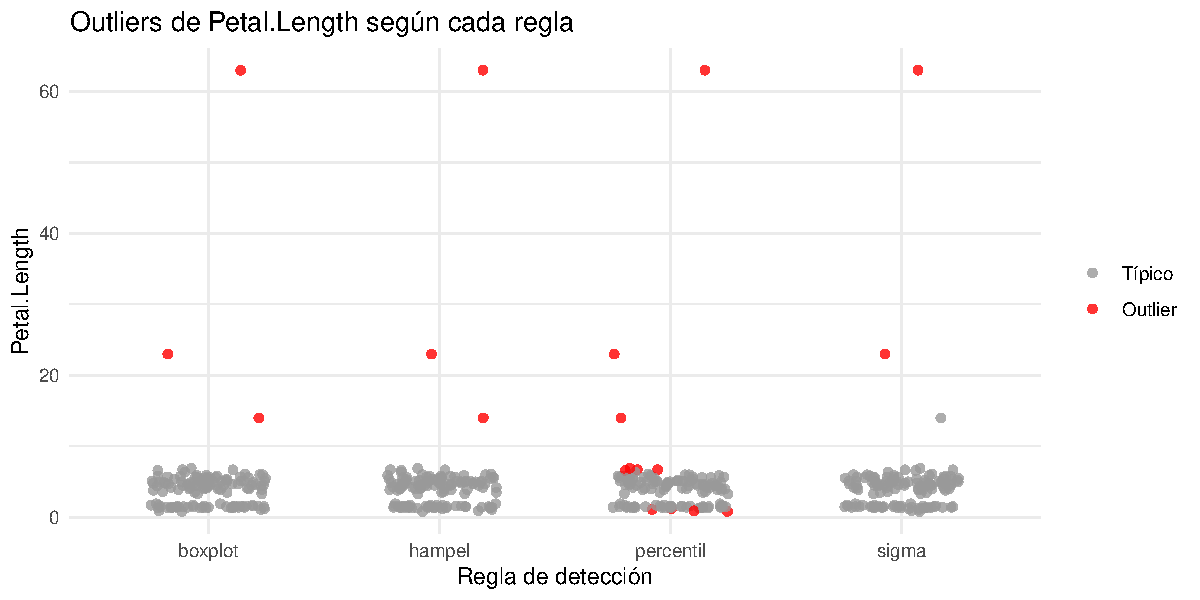
\includegraphics{./figure/Solucion ejercicio 8-1} \end{center}

\section{Imputación de datos}\label{imputaciuxf3n-de-datos}

Como se ha visto, con \emph{missing data} nos referimos a una
observación (o conjunto de observaciones) cuyo valor no es conocido.

Vamos a ver a continuación ejemplos de cómo imputar valores realistas a
esas observaciones perdidas.

\subsection{Ejercicio 9: Imputación de datos perdidos con estadísticos
básicos}\label{ejercicio-9-imputaciuxf3n-de-datos-perdidos-con-estaduxedsticos-buxe1sicos}

La opción más sencilla es imputar con un valor estimado de los valores
conocidos (por ejemplo, con la media, la mediana, o la moda).

Se puede realizar una imputación generalizada (usando todos los valores
de la variable) o una imputación a partir de casos similares (la
estimación se realiza teniendo en cuenta otra variable):

\begin{itemize}
\tightlist
\item
  Imputa los missing data en \texttt{Petal.Length} empleando la media.
  Nota: Puedes reemplazar los valores vacios usando \texttt{mutate} con
  \texttt{ifelse} creando una nueva variable \texttt{Petal.Length1}.
\end{itemize}

\begin{Shaded}
\begin{Highlighting}[]
\CommentTok{\# "imputado" marca qué valores eran NA originalmente }
\NormalTok{iris\_imp }\OtherTok{\textless{}{-}}\NormalTok{ dirty\_iris }\SpecialCharTok{\%\textgreater{}\%}
  \FunctionTok{mutate}\NormalTok{(}\AttributeTok{imputado =} \FunctionTok{is.na}\NormalTok{(Petal.Length),}
         \AttributeTok{Petal.Length1 =} \FunctionTok{ifelse}\NormalTok{(}\FunctionTok{is.na}\NormalTok{(Petal.Length),}
                                \FunctionTok{mean}\NormalTok{(Petal.Length, }\AttributeTok{na.rm =} \ConstantTok{TRUE}\NormalTok{),}
\NormalTok{                                Petal.Length))}

\CommentTok{\# Valor con el que se ha imputado}
\FunctionTok{mean}\NormalTok{(dirty\_iris}\SpecialCharTok{$}\NormalTok{Petal.Length, }\AttributeTok{na.rm =} \ConstantTok{TRUE}\NormalTok{)}
\end{Highlighting}
\end{Shaded}

\begin{verbatim}
[1] 4.484192
\end{verbatim}

\begin{itemize}
\tightlist
\item
  Imputa los missing data en \texttt{Petal.Length} empleando en esta
  ocasión la media para cada tipo de \texttt{Species}
  (usar\texttt{group\_by} y \texttt{mutate}) creando una nueva variable
  \texttt{Petal.Length2}.
\end{itemize}

\begin{Shaded}
\begin{Highlighting}[]
\NormalTok{iris\_imp }\OtherTok{\textless{}{-}}\NormalTok{ iris\_imp }\SpecialCharTok{\%\textgreater{}\%}
  \FunctionTok{group\_by}\NormalTok{(Species) }\SpecialCharTok{\%\textgreater{}\%}
  \FunctionTok{mutate}\NormalTok{(}\AttributeTok{Petal.Length2 =} \FunctionTok{ifelse}\NormalTok{(}\FunctionTok{is.na}\NormalTok{(Petal.Length),}
                                \FunctionTok{mean}\NormalTok{(Petal.Length, }\AttributeTok{na.rm =} \ConstantTok{TRUE}\NormalTok{),}
\NormalTok{                                Petal.Length)) }\SpecialCharTok{\%\textgreater{}\%}
  \FunctionTok{ungroup}\NormalTok{()}

\CommentTok{\# Medias por especie usadas en la imputación}
\NormalTok{iris\_imp }\SpecialCharTok{\%\textgreater{}\%}
  \FunctionTok{group\_by}\NormalTok{(Species) }\SpecialCharTok{\%\textgreater{}\%}
  \FunctionTok{summarise}\NormalTok{(}\AttributeTok{media =} \FunctionTok{mean}\NormalTok{(Petal.Length, }\AttributeTok{na.rm =} \ConstantTok{TRUE}\NormalTok{), }\AttributeTok{n\_NA =} \FunctionTok{sum}\NormalTok{(imputado))}
\end{Highlighting}
\end{Shaded}

\begin{verbatim}
# A tibble: 3 x 3
  Species    media  n_NA
  <chr>      <dbl> <int>
1 setosa      1.80    10
2 versicolor  4.55     5
3 virginica   6.80     5
\end{verbatim}

\begin{Shaded}
\begin{Highlighting}[]
\NormalTok{iris\_imp }\SpecialCharTok{\%\textgreater{}\%} \FunctionTok{select}\NormalTok{(Species, Petal.Length, Petal.Length1, Petal.Length2) }\SpecialCharTok{\%\textgreater{}\%}
  \FunctionTok{filter}\NormalTok{(}\FunctionTok{is.na}\NormalTok{(Petal.Length)) }\SpecialCharTok{\%\textgreater{}\%} \FunctionTok{head}\NormalTok{(}\DecValTok{8}\NormalTok{)}
\end{Highlighting}
\end{Shaded}

\begin{verbatim}
# A tibble: 8 x 4
  Species    Petal.Length Petal.Length1 Petal.Length2
  <chr>             <dbl>         <dbl>         <dbl>
1 setosa               NA          4.48          1.80
2 setosa               NA          4.48          1.80
3 setosa               NA          4.48          1.80
4 virginica            NA          4.48          6.80
5 setosa               NA          4.48          1.80
6 versicolor           NA          4.48          4.55
7 setosa               NA          4.48          1.80
8 setosa               NA          4.48          1.80
\end{verbatim}

\subsection{Ejercicio 10: Representación
gráfica}\label{ejercicio-10-representaciuxf3n-gruxe1fica}

Vamos a comparar ahora los dos métodos de imputación gráficamente
eliminando los outliers para una mejor visualización.

\begin{itemize}
\tightlist
\item
  Recalcula las reglas de identificación de outliers (Ejercicio 6) para
  la nueva variable \texttt{Petal.Length2}.
\end{itemize}

\begin{Shaded}
\begin{Highlighting}[]
\NormalTok{iris\_imp }\OtherTok{\textless{}{-}}\NormalTok{ iris\_imp }\SpecialCharTok{\%\textgreater{}\%}
  \FunctionTok{mutate}\NormalTok{(}\FunctionTok{across}\NormalTok{(Petal.Length2,}
                \FunctionTok{list}\NormalTok{(}\AttributeTok{sigma     =}\NormalTok{ reglasigma,}
                     \AttributeTok{hampel    =}\NormalTok{ reglahampel,}
                     \AttributeTok{boxplot   =}\NormalTok{ reglaboxplot,}
                     \AttributeTok{percentil =}\NormalTok{ reglapercentil),}
                \AttributeTok{.names =} \StringTok{"out2\_\{.fn\}"}\NormalTok{))}

\CommentTok{\# Outliers detectados en Petal.Length2 por cada regla}
\NormalTok{iris\_imp }\SpecialCharTok{\%\textgreater{}\%} \FunctionTok{summarise}\NormalTok{(}\FunctionTok{across}\NormalTok{(}\FunctionTok{starts\_with}\NormalTok{(}\StringTok{"out2\_"}\NormalTok{), }\SpecialCharTok{\textasciitilde{}} \FunctionTok{sum}\NormalTok{(.x, }\AttributeTok{na.rm =} \ConstantTok{TRUE}\NormalTok{)))}
\end{Highlighting}
\end{Shaded}

\begin{verbatim}
# A tibble: 1 x 4
  out2_sigma out2_hampel out2_boxplot out2_percentil
       <int>       <int>        <int>          <int>
1          2           3            3              8
\end{verbatim}

\begin{itemize}
\tightlist
\item
  Representa los dos tipos de imputación empleados en un gráfico de
  dispersión (\texttt{Petal.Length1} vs.~\texttt{Petal.Length2})
  eliminando los outliers identificados con la regla
  \texttt{reglapercentil} y poniendo en diferente color los datos
  originales y los imputados.
\end{itemize}

\begin{Shaded}
\begin{Highlighting}[]
\NormalTok{iris\_imp }\SpecialCharTok{\%\textgreater{}\%}
  \FunctionTok{filter}\NormalTok{(}\SpecialCharTok{!}\NormalTok{out2\_percentil) }\SpecialCharTok{\%\textgreater{}\%}
  \FunctionTok{mutate}\NormalTok{(}\AttributeTok{tipo =} \FunctionTok{ifelse}\NormalTok{(imputado, }\StringTok{"Imputado"}\NormalTok{, }\StringTok{"Original"}\NormalTok{)) }\SpecialCharTok{\%\textgreater{}\%}
  \FunctionTok{ggplot}\NormalTok{(}\FunctionTok{aes}\NormalTok{(}\AttributeTok{x =}\NormalTok{ Petal.Length1, }\AttributeTok{y =}\NormalTok{ Petal.Length2, }\AttributeTok{color =}\NormalTok{ tipo)) }\SpecialCharTok{+}
  \FunctionTok{geom\_point}\NormalTok{(}\AttributeTok{alpha =} \FloatTok{0.8}\NormalTok{, }\AttributeTok{size =} \DecValTok{2}\NormalTok{) }\SpecialCharTok{+}
  \FunctionTok{scale\_color\_manual}\NormalTok{(}\AttributeTok{values =} \FunctionTok{c}\NormalTok{(}\StringTok{"Original"} \OtherTok{=} \StringTok{"grey60"}\NormalTok{, }\StringTok{"Imputado"} \OtherTok{=} \StringTok{"red"}\NormalTok{)) }\SpecialCharTok{+}
  \FunctionTok{labs}\NormalTok{(}\AttributeTok{title =} \StringTok{"Imputación con la media global vs. media por especie"}\NormalTok{,}
       \AttributeTok{subtitle =} \StringTok{"Sin outliers según la regla de percentiles"}\NormalTok{,}
       \AttributeTok{x =} \StringTok{"Petal.Length1 (media global)"}\NormalTok{,}
       \AttributeTok{y =} \StringTok{"Petal.Length2 (media por especie)"}\NormalTok{, }\AttributeTok{color =} \ConstantTok{NULL}\NormalTok{) }\SpecialCharTok{+}
  \FunctionTok{theme\_minimal}\NormalTok{()}
\end{Highlighting}
\end{Shaded}

\begin{center}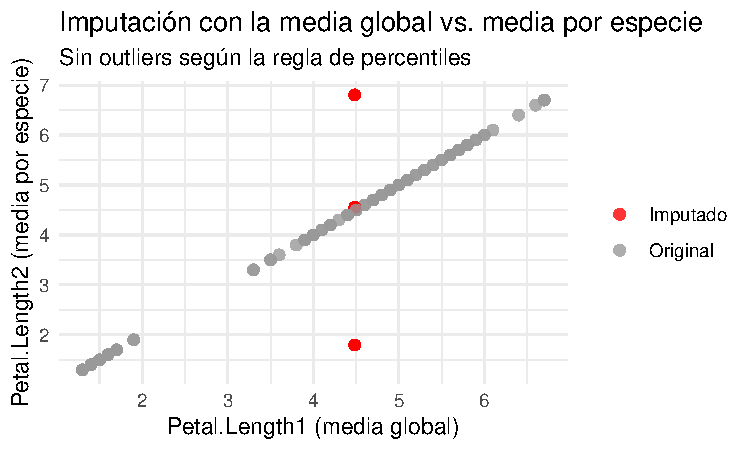
\includegraphics{./figure/Solucion ejercicio 10b-1} \end{center}

\end{document}
